% Source: Code/ML_overlay/ir_rgb_registration/paper/ml_overlay_report_materials/ir_rgb_registration_report/figures/fig_ablation_study_design.tex
\documentclass[tikz,border=10pt]{standalone}
\usepackage{tikz}
\usetikzlibrary{matrix,positioning,shapes.geometric}

\definecolor{Garnet}{RGB}{115,0,10}
\definecolor{Rose}{RGB}{204,46,64}
\definecolor{Atlantic}{RGB}{70,106,159}
\definecolor{Congaree}{RGB}{31,65,77}
\definecolor{Horseshoe}{RGB}{101,120,11}
\definecolor{Black90}{RGB}{54,54,54}
\definecolor{Black70}{RGB}{92,92,92}
\definecolor{White}{RGB}{255,255,255}

\begin{document}
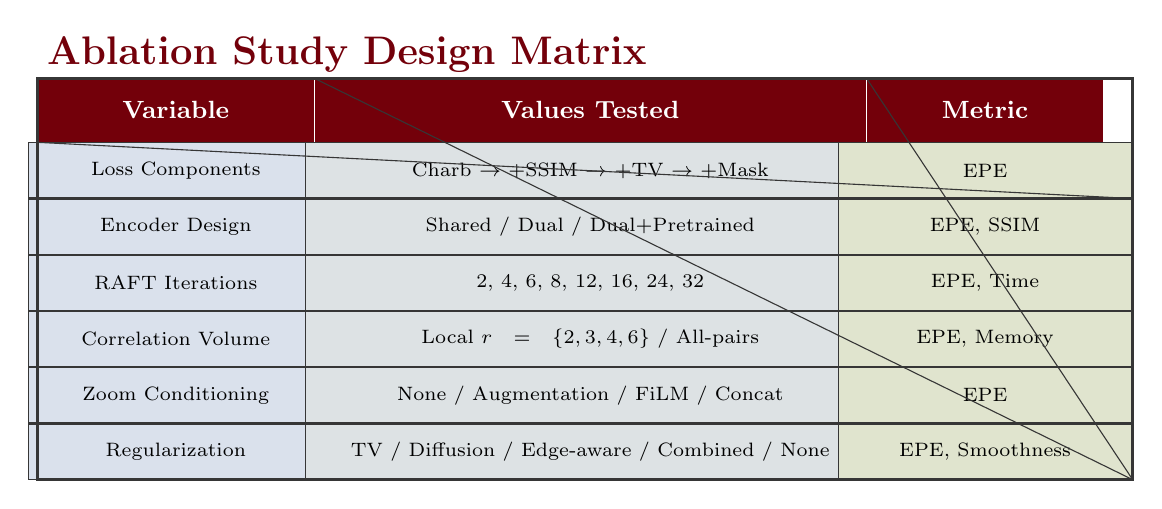
\begin{tikzpicture}[
    header/.style={fill=Garnet,text=White,font=\bfseries\small,minimum height=0.8cm},
    cell/.style={draw=Black90,minimum height=0.7cm,text width=3.5cm,align=center,font=\scriptsize},
    varcell/.style={cell,fill=Atlantic!20},
    valcell/.style={cell,fill=Congaree!15},
    metcell/.style={cell,fill=Horseshoe!20}
]

% Header row
\node[header,minimum width=3.5cm] (h1) at (0,0) {Variable};
\node[header,minimum width=7cm,anchor=west] (h2) at (h1.east) {Values Tested};
\node[header,minimum width=3cm,anchor=west] (h3) at (h2.east) {Metric};

% Row 1: Loss Components
\node[varcell,below=0cm of h1,anchor=north] (v1) {Loss Components};
\node[valcell,below=0cm of h2,anchor=north,text width=7cm] (t1) {Charb $\rightarrow$ +SSIM $\rightarrow$ +TV $\rightarrow$ +Mask};
\node[metcell,below=0cm of h3,anchor=north,minimum width=3cm] (m1) {EPE};

% Row 2: Encoder Design
\node[varcell,below=0cm of v1,anchor=north] (v2) {Encoder Design};
\node[valcell,below=0cm of t1,anchor=north,text width=7cm] (t2) {Shared / Dual / Dual+Pretrained};
\node[metcell,below=0cm of m1,anchor=north,minimum width=3cm] (m2) {EPE, SSIM};

% Row 3: RAFT Iterations
\node[varcell,below=0cm of v2,anchor=north] (v3) {RAFT Iterations};
\node[valcell,below=0cm of t2,anchor=north,text width=7cm] (t3) {2, 4, 6, 8, 12, 16, 24, 32};
\node[metcell,below=0cm of m2,anchor=north,minimum width=3cm] (m3) {EPE, Time};

% Row 4: Correlation Volume
\node[varcell,below=0cm of v3,anchor=north] (v4) {Correlation Volume};
\node[valcell,below=0cm of t3,anchor=north,text width=7cm] (t4) {Local $r=\{2,3,4,6\}$ / All-pairs};
\node[metcell,below=0cm of m3,anchor=north,minimum width=3cm] (m4) {EPE, Memory};

% Row 5: Zoom Conditioning
\node[varcell,below=0cm of v4,anchor=north] (v5) {Zoom Conditioning};
\node[valcell,below=0cm of t4,anchor=north,text width=7cm] (t5) {None / Augmentation / FiLM / Concat};
\node[metcell,below=0cm of m4,anchor=north,minimum width=3cm] (m5) {EPE};

% Row 6: Regularization
\node[varcell,below=0cm of v5,anchor=north] (v6) {Regularization};
\node[valcell,below=0cm of t5,anchor=north,text width=7cm] (t6) {TV / Diffusion / Edge-aware / Combined / None};
\node[metcell,below=0cm of m5,anchor=north,minimum width=3cm] (m6) {EPE, Smoothness};

% Draw borders
\draw[Black90,line width=1pt] (h1.north west) rectangle (m6.south east);
\draw[Black90] (h1.south west) -- (m1.south east);
\draw[Black90] (v1.south west) -- (m1.south east);
\draw[Black90] (v2.south west) -- (m2.south east);
\draw[Black90] (v3.south west) -- (m3.south east);
\draw[Black90] (v4.south west) -- (m4.south east);
\draw[Black90] (v5.south west) -- (m5.south east);
\draw[Black90] (h1.north east) -- (m6.south east);
\draw[Black90] (h2.north east) -- (m6.south east);

% Title
\node[font=\Large\bfseries,Garnet,above=0.3cm of h1.north west,anchor=west] {Ablation Study Design Matrix};

\end{tikzpicture}
\end{document}
